% ----------------------------------------------------------------------%
% Coquille pour thèses et mémoires.                                     %
% UQAR, 29 mai 2009.                                                    %
% Modifié par F. Cyr - aout 2013                                        %
%		 AC. Tassel - janvier 2014                                          %
%		 C. Rigaud - 2014-2015                                              %
% ----------------------------------------------------------------------%

% ----------------------------------------------------------------------%
% Kevin Cazelles: J'ai utilisé ce template car c'est ce que j'ai utilisé
%  pour ma thèse
% ----------------------------------------------------------------------%



% ----------------------------------------------------------------------%
% 1- Préambule.                                                        %
% ----------------------------------------------------------------------%

% Pour le dépôt initial (recto), utiliser oneside.
% Pour le dépôt final  (recto-verso), remplacer oneside par twoside.

\documentclass[12pt,oneside,francais,letterpaper]{stylethese}
% \documentclass[12pt,twoside,letterpaper]{stylethese}

\raggedbottom % Évite les espaces trop gands entre chaque section.

% \usepackage{multirow}
\usepackage{natbib}
\usepackage{amssymb,amsmath}
\usepackage{enumerate} % For fancy enumerate item labels.
% \usepackage{utopia}
\usepackage{txfonts,empheq}
%\usepackage{chancery}
%\usepackage{ccaption}		 %pour utiliser \legend (pour l'explication de la figure,texte plus long)
%\usepackage{pgfplots}      	 % dessiner des graphes direct dans LaTeX
%\pgfplotsset{compat=1.3}
\usepackage{multicol}

\usepackage[utf8x]{inputenc}
\usepackage{ucs}


\usepackage{chapterbib} % <----- for bibliography per chapter
%\usepackage[duplicate]{chapterbib}
%\usepackage{url}

% Ajout Cyril :
\usepackage[linktocpage=true,linkcolor=cyan,citecolor=cyan,colorlinks=true,urlcolor=blue,pagebackref]{hyperref}
\usepackage[english,french]{cleveref}
\usepackage{upgreek}
\usepackage{textcomp}
\usepackage{tabularx}
\usepackage{longtable}
\usepackage{ltxtable}
\usepackage{pdflscape}
\usepackage{booktabs}
\usepackage{afterpage}
\usepackage{floatpag}
\usepackage[babel=true]{csquotes}
\usepackage{pifont}
\usepackage{soulutf8}
\usepackage{caption}
\usepackage{color}
\usepackage{ulem}


%%------------------ Ajout Kevin Cazelles
%%------------------ Ce qu'on a besoin pour inclure du code
%%------------------ => c'est ce qu'utilise pandoc pour faire mettre en page les
%%------------------ des code chunk (pour l'obtenir, voir template ou faire
%%------------------ un exemple minimal avec du code en md puis le convertir en
%%------------------ Latex avec l'option standalone (option -s))
\usepackage{lmodern}
% \usepackage{ifxetex,ifluatex}
% \usepackage{fixltx2e} % provides \textsubscript
% \ifnum 0\ifxetex 1\fi\ifluatex 1\fi=0 % if pdftex
%   \usepackage[T1]{fontenc}
%   \usepackage[utf8]{inputenc}
% \else % if luatex or xelatex
%   \ifxetex
%     \usepackage{mathspec}
%   \else
%     \usepackage{fontspec}
%   \fi
%   \defaultfontfeatures{Ligatures=TeX,Scale=MatchLowercase}
% \fi
% use upquote if available, for straight quotes in verbatim environments
\IfFileExists{upquote.sty}{\usepackage{upquote}}{}
% use microtype if available
\IfFileExists{microtype.sty}{%
\usepackage[]{microtype}
\UseMicrotypeSet[protrusion]{basicmath} % disable protrusion for tt fonts
}{}
\PassOptionsToPackage{hyphens}{url} % url is loaded by hyperref
% \usepackage[unicode=true]{hyperref}
% \hypersetup{pdfborder={0 0 0}, breaklinks=true}
\urlstyle{same}  % don't use monospace font for urls
\usepackage{fancyvrb}
\newcommand{\VerbBar}{|}
\newcommand{\VERB}{\Verb[commandchars=\\\{\}]}
\DefineVerbatimEnvironment{Highlighting}{Verbatim}{commandchars=\\\{\}}
% Add ',fontsize=\small' for more characters per line
\newenvironment{Shaded}{}{}
\newcommand{\KeywordTok}[1]{\textcolor[rgb]{0.00,0.44,0.13}{\textbf{#1}}}
\newcommand{\DataTypeTok}[1]{\textcolor[rgb]{0.56,0.13,0.00}{#1}}
\newcommand{\DecValTok}[1]{\textcolor[rgb]{0.25,0.63,0.44}{#1}}
\newcommand{\BaseNTok}[1]{\textcolor[rgb]{0.25,0.63,0.44}{#1}}
\newcommand{\FloatTok}[1]{\textcolor[rgb]{0.25,0.63,0.44}{#1}}
\newcommand{\ConstantTok}[1]{\textcolor[rgb]{0.53,0.00,0.00}{#1}}
\newcommand{\CharTok}[1]{\textcolor[rgb]{0.25,0.44,0.63}{#1}}
\newcommand{\SpecialCharTok}[1]{\textcolor[rgb]{0.25,0.44,0.63}{#1}}
\newcommand{\StringTok}[1]{\textcolor[rgb]{0.25,0.44,0.63}{#1}}
\newcommand{\VerbatimStringTok}[1]{\textcolor[rgb]{0.25,0.44,0.63}{#1}}
\newcommand{\SpecialStringTok}[1]{\textcolor[rgb]{0.73,0.40,0.53}{#1}}
\newcommand{\ImportTok}[1]{#1}
\newcommand{\CommentTok}[1]{\textcolor[rgb]{0.38,0.63,0.69}{\textit{#1}}}
\newcommand{\DocumentationTok}[1]{\textcolor[rgb]{0.73,0.13,0.13}{\textit{#1}}}
\newcommand{\AnnotationTok}[1]{\textcolor[rgb]{0.38,0.63,0.69}{\textbf{\textit{#1}}}}
\newcommand{\CommentVarTok}[1]{\textcolor[rgb]{0.38,0.63,0.69}{\textbf{\textit{#1}}}}
\newcommand{\OtherTok}[1]{\textcolor[rgb]{0.00,0.44,0.13}{#1}}
\newcommand{\FunctionTok}[1]{\textcolor[rgb]{0.02,0.16,0.49}{#1}}
\newcommand{\VariableTok}[1]{\textcolor[rgb]{0.10,0.09,0.49}{#1}}
\newcommand{\ControlFlowTok}[1]{\textcolor[rgb]{0.00,0.44,0.13}{\textbf{#1}}}
\newcommand{\OperatorTok}[1]{\textcolor[rgb]{0.40,0.40,0.40}{#1}}
\newcommand{\BuiltInTok}[1]{#1}
\newcommand{\ExtensionTok}[1]{#1}
\newcommand{\PreprocessorTok}[1]{\textcolor[rgb]{0.74,0.48,0.00}{#1}}
\newcommand{\AttributeTok}[1]{\textcolor[rgb]{0.49,0.56,0.16}{#1}}
\newcommand{\RegionMarkerTok}[1]{#1}
\newcommand{\InformationTok}[1]{\textcolor[rgb]{0.38,0.63,0.69}{\textbf{\textit{#1}}}}
\newcommand{\WarningTok}[1]{\textcolor[rgb]{0.38,0.63,0.69}{\textbf{\textit{#1}}}}
\newcommand{\AlertTok}[1]{\textcolor[rgb]{1.00,0.00,0.00}{\textbf{#1}}}
\newcommand{\ErrorTok}[1]{\textcolor[rgb]{1.00,0.00,0.00}{\textbf{#1}}}
\newcommand{\NormalTok}[1]{#1}
\IfFileExists{parskip.sty}{%
\usepackage{parskip}
}{% else
\setlength{\parindent}{0pt}
\setlength{\parskip}{6pt plus 2pt minus 1pt}
}
\setlength{\emergencystretch}{3em}  % prevent overfull lines
\providecommand{\tightlist}{%
  \setlength{\itemsep}{0pt}\setlength{\parskip}{0pt}}
\setcounter{secnumdepth}{0}
% Redefines (sub)paragraphs to behave more like sections
\ifx\paragraph\undefined\else
\let\oldparagraph\paragraph
\renewcommand{\paragraph}[1]{\oldparagraph{#1}\mbox{}}
\fi
\ifx\subparagraph\undefined\else
\let\oldsubparagraph\subparagraph
\renewcommand{\subparagraph}[1]{\oldsubparagraph{#1}\mbox{}}
\fi



\captionsetup{singlelinecheck=false}
% \captionsetup{singlelinecheck=false}

% Taille des légendes des 'Long Tables'
\setlength{\LTcapwidth}{\linewidth}
% \setlength{\LTcapwidth}{1.5\linewidth} 



%Marge inférieure avec note de bas de page
\setlength{\footnotesep}{1cm}

%Régler le problème des Et/And entre deux auteurs (voir le fichier "tutoriel bst")
\newcommand*{\andname}{and}
      \addto \captionsenglish {\renewcommand*{\andname}{and}}
      \addto \captionsfrench  {\renewcommand*{\andname}{et}}

%Intitulé des figures en français
\addto\captionsfrench{\renewcommand{\figurename}{Figure}}

%Intitulé des tableaux en français
\addto\captionsfrench{\renewcommand{\tablename}{Tableau}}

% Interligne 1 et 1/2.
\setstretch{1.5}

% Pour créer un index (optionnel).
\makeindex

% Info sur la thèse (Titre, auteur, etc.)
\Titre{LE TITRE DE LA THÈSE}
% Mettre en majuscule!!
\Auteur{David Beauchesnes}
\Faculte{programme de doctorat en Biologie}
\Diplome{Philosophiae Doctor}
\Date{Septembre}{2017}



\These


\Articles



\begin{document}
\pdfstringdefDisableCommands{%
\let\MakeUppercase\relax}



% ----------------------------------------------------------------------%
% 2- Liminaires de la thèse.                                            %
% ----------------------------------------------------------------------%

%----------------------------------------------------------------------%
% Liminaires de la thèse.                                              %
% UQAR septembre 2013                                                  %
% ---------------------------------------------------------------------%

% ----------------------------------------------------------------------%
% 1- Page titre.                                                        %
% ----------------------------------------------------------------------%


\Pagetitre
\cleardoublepage
% ----------------------------------------------------------------------%
% inclusions qui pourraient mériter d'être incluses dans le .cls
% (commentez si non-nécessaire)
% 1.1 - Composition du Jury.                                           %
%\thispagestyle{empty}

\null
\vfill
\noindent \textbf{Composition du jury:}\\
\vspace{1cm}

\begin{singlespace}
  \noindent \textbf{QQ1, président du jury, Université du Québec à Montréal}\\

  \noindent \textbf{Dominique Gravel, directeur de recherche, Université du Québec à Rimouski}\\

  \noindent \textbf{Phillipe Archambault, directeur de recherche, Université de Montpellier}\\

  \noindent \textbf{QQ1, examinateur interne, QQpart}\\

  \noindent \textbf{Q1, examinateur interne, Université du Québec à Rimouski}\\

  \noindent \textbf{QQ1, examinateur externe, QQpart}\\
\end{singlespace}

\vspace{2cm}
\noindent Dépôt initial le 12 septembre 2017
\hspace{3cm}
Dépôt final le [-]


\cleardoublepage

% % 1.2 - Avertissement biblio.
%\thispagestyle{empty}

\vspace{2cm}
\begin{center}
UNIVERSITÉ DU QUÉBEC À RIMOUSKI\\
Service de la bibliothèque
\end{center}

\vspace{3cm}
\begin{center}
Avertissement
\end{center}


\vspace{1cm}

\noindent La diffusion de ce mémoire ou de cette thèse se fait dans le respect des droits de son auteur, qui a signé le formulaire {\itshape \og Autorisation de reproduire et de diffuser un rapport, un mémoire ou une thèse \fg}. 
En signant ce formulaire, l’auteur concède à l’Université du Québec à Rimouski une licence non exclusive d’utilisation et de publication de la totalité ou d’une partie importante de son travail de recherche pour des fins pédagogiques et non commerciales. 
Plus précisément, l’auteur autorise l’Université du Québec à Rimouski à reproduire, diffuser, prêter, distribuer ou vendre des copies de son travail de recherche à des fins non commerciales sur quelque support que ce soit, y compris l’Internet. 
Cette licence et cette autorisation n’entraînent pas une renonciation de la part de l’auteur à ses droits moraux ni à ses droits de propriété intellectuelle. 
Sauf entente contraire, l’auteur conserve la liberté de diffuser et de commercialiser ou non ce travail dont il possède un exemplaire.



\cleardoublepage
% % 1.3 - Dedicace.
%\thispagestyle{empty}

\begin{minipage}[l]{0.45\textwidth}

\end{minipage}%
\hfill
\begin{minipage}[r]{0.5\textwidth}
\begin{quotation}
\begin{doublespace}

à qui tu veux,

\end{doublespace}
\end{quotation}
\end{minipage}%

\cleardoublepage

% ----------------------------------------------------------------------%


% ----------------------------------------------------------------------%
% 2- Remerciements.                                                    %
% ----------------------------------------------------------------------%

\remerciements
\selectlanguage{frenchb}
La j'ai fait des mercis personnels


% [Cette page est facultative; l’éliminer si elle n’est pas utilisée. Les remerciements peuvent aussi être intégrés à l'avant-propos. C’est dans cette section que l’on remercie les personnes qui ont contribué au projet, les organismes ou les entreprises subventionnaires qui ont soutenu financièrement le projet.]



% ----------------------------------------------------------------------%
% 3- Avant-propos.                                                     %
% ----------------------------------------------------------------------%

\avantpropos
\selectlanguage{frenchb}
La j'ai fait des merci formels!



% [Cette page est facultative; l’éliminer si elle n’est pas utilisée. L’avant-propos ne doit pas être confondu avec l'introduction. Il n’est pas d’ordre scientifique alors que l’introduction l’est. Il s’agit d'un discours préliminaire qui permet notamment à l'auteur d'exposer les raisons qui l'ont amené à étudier le sujet choisi, le but qu'il veut atteindre, ainsi que les possibilités et les limites de son travail. On peut inclure les remerciements à la fin de ce texte au lieu de les présenter sur une page distincte.]



% ----------------------------------------------------------------------%
% 4- Resume/Abstract                                                           %
% ----------------------------------------------------------------------%

\resume
\begin{singlespace}
La biogéographie est l'étude des mécanismes et des processus qui
influencent la répartition géographique des être vivants. B

\begin{quote}
Mots clés: Biogéographie, interactions biotiques, réseaux écologiques,
contraintes abiotiques, co-occurrence, théorie de la biogéographie des
îles, théorie métabolique de l'écologie.
\end{quote}

  % [Le résumé en français doit présenter en 350 mots maximum pour un mémoire et en 700 mots pour une thèse : (1) le but de la recherche, (2) les sujets étudiés, (3) les hypothèses de travail et la méthode utilisée, (4) les principaux résultats et (5) les conclusions de l'étude ou de la recherche.]

\end{singlespace}
\cleardoublepage


\abstract
\begin{singlespace}
Biogeography is the study of the mechanisms and processes that control
the geographical distribution of plants and animals.

\begin{quote}
Keywords: Biogeography, biotic interactions, ecological networks,
abiotic constrains, co-occurrence, theory of island biogeography,
metabolic theory of ecology.
\end{quote}


  % [L'abstract doit être une traduction anglaise fidèle et grammaticalement correcte du résumé en français.]

\end{singlespace}
\cleardoublepage




% ----------------------------------------------------------------------%
% 5- Table des matières.                                               %
% ----------------------------------------------------------------------%

\tabledesmatieres



% ----------------------------------------------------------------------%
% 6- Liste des tableaux.                                               %
% ----------------------------------------------------------------------%

\listedestableaux

% ----------------------------------------------------------------------%
% 7- Table des matières.                                               %
% ----------------------------------------------------------------------%

\listedesfigures

% ----------------------------------------------------------------------%
% 8- Liste des abréviations (optionnel).                               %
% ----------------------------------------------------------------------%

\listeabrev
\begin{liste}

\item[DOI]~: \textit{Digital Object Identifier}; identifiant numérique d'objet.

\item[GIEC]~: Groupe d'experts Intergouvernemental sur l'Évolution du Climat.

\item[IPBES]~: \textit{Intergovernmental Science-Policy Platform on Biodiversity and Ecosystem Services}; Plateforme intergouvernementale sur la biodiversité et les services écosystémiques.

\end{liste}



% ----------------------------------------------------------------------%
% 9- Liste des symboles (optionnel).                                   %
% ----------------------------------------------------------------------%

% \listesymboles
% \begin{liste}
% \item[SYMBOLE 1] Ceci est la définition du symbole 1.
%
% \item[SYMBOLE 2] Ceci est la définition du symbole 2.
%
% \item[SYMBOLE 3] Ceci est la définition du symbole 3.
% \end{liste}

% ----------------------------------------------------------------------%
% Fin des liminaires.                                                  %
% ----------------------------------------------------------------------%

\cleardoublepage







% ----------------------------------------------------------------------%
% 3- Corps de la thèse.                                                %
% ----------------------------------------------------------------------%

\debutcorps
\cleardoublepage
% Utiliser      chapitres.tex pour une thèse (ou mémoire) traditionnelle.
% Remplacer par articles.tex  pour une thèse (ou mémoire) par articles.


\introduction
\selectlanguage{french}

% \chapter{INTRODUCTION GÉNÉRALE}
\section*{Titre de niveau 1}\label{titre-de-niveau-1}
\addcontentsline{toc}{section}{Titre de niveau 1}

Note: Le \{-\} dans le fichier .md signal que la section ne sera pas
numérotée.

\subsection*{Titre de niveau 2}\label{titre-de-niveau-2}
\addcontentsline{toc}{subsection}{Titre de niveau 2}

\subsubsection*{Titre de niveau 3}\label{titre-de-niveau-3}
\addcontentsline{toc}{subsubsection}{Titre de niveau 3}

\section{Quelques rappels sur Makdown et
Pandoc}\label{quelques-rappels-sur-makdown-et-pandoc}

Pour la synthaxe, ci-dessous est présenté ``l'essentiel'' pour la
rédaction d'un document tel une thèse. Pour avoir des informations plus
exhaustives et pour bien comprendre ce qu'est Markdown, voir la
\href{http://spec.commonmark.org/0.25/}{dernière spécifcation de Common
Mark}.

Pour convertir le fichier Markdown (.md) en fichier Latex (.tex),
j'utilise le converteur universel de documeent
\href{http://pandoc.org}{Pandoc}.

\section*{Synthaxe Pandoc Markdown}\label{synthaxe-pandoc-markdown}
\addcontentsline{toc}{section}{Synthaxe Pandoc Markdown}

\subsection*{Simple mise en forme}\label{simple-mise-en-forme}
\addcontentsline{toc}{subsection}{Simple mise en forme}

Écrire en \textbf{gras} utiliser un ``\textbackslash{}emph'':
\emph{emph} (en français c'est souligner en anglais c'est en italic).
Utiliser un \textsuperscript{exposant}. Utiliser un
\textsubscript{indice} on peut même \sout{barrer}. Pour faire une
énumération (hyphenation)~:

\begin{itemize}
\tightlist
\item
  cool
\item
  cool2
\end{itemize}

une liste numérotée~:

\begin{enumerate}
\def\labelenumi{\arabic{enumi}.}
\tightlist
\item
  cool
\item
  cool2
\end{enumerate}

\subsection{Note de bas de page}\label{note-de-bas-de-page}

Une note de bas de page\footnote{Ici, mettre le texte de la note de bas
  de page.}. Noter on peut les regrouper n'importe où dans le document.

\subsection{Liens hypertextes}\label{liens-hypertextes}

Une lien internet {[}nom du lien{]}(adresse su lien), ex:
\href{http://pandoc.org}{Pandoc}.

\subsection*{Citations}\label{citations}
\addcontentsline{toc}{subsection}{Citations}

Pour les citation courtes en anglais les guillemets anglais ``That's one
small step for man, one giant leap for mankind''. Pour les français, le
mieux utilser les codes HTML: « Vive le Québec libre! »

Pour faire une citation plus longue, il suffit d'utiliser
`\textgreater{}' citation de plus de 2 lignes:

\begin{quote}
Lorem ipsum dolor sit amet, consectetur adipisicing elit, sed do eiusmod
tempor incididunt ut labore et dolore magna aliqua. Ut enim ad minim
veniam, quis nostrud exercitation ullamco laboris nisi ut aliquip ex ea
commodo consequat. Duis aute irure dolor in reprehenderit in voluptate
velit esse cillum dolore eu fugiat nulla pariatur. Excepteur sint
occaecat cupidatat non proident, sunt in culpa qui officia deserunt
mollit anim id est laborum.
\end{quote}

\subsection*{Symboles mathématques et
équations}\label{symboles-mathuxe9matques-et-uxe9quations}
\addcontentsline{toc}{subsection}{Symboles mathématques et équations}

\subsubsection*{En ligne}\label{en-ligne}
\addcontentsline{toc}{subsubsection}{En ligne}

\$votre equation\$ Après il faut connaître les symboles latex. Il y a
plein de référence en ligne, par exemple sur
\href{https://en.wikibooks.org/wiki/LaTeX/Mathematics}{Wikilivres}

Exemple: \(\overline{x}\), \(\mathcal{N}\)

\subsubsection*{Équations}\label{uxe9quations}
\addcontentsline{toc}{subsubsection}{Équations}

Utiliser \$\$votre equation\$\$ pour insérer une équations. Pour faire
des références aux équations insérées, j'utilise un filtre pandoc
\href{https://github.com/tomduck/pandoc-eqnos}{Pandoc-eqnos} (écrit en
python). Par exemple~:

\begin{equation}\prod_{i=1}^nu_n=1\label{eq:intr_1}\end{equation}

Voila, une référence à l'équation \ref{eq:intr_1}. Vous pouvez mettre
des équations les unes à la suite des autres, elles seront alors
considérées comme deux équations indpendantes.

\begin{equation}\sum_{i=1}^nu_n=1\label{eq:intr_2}\end{equation}
\begin{equation}\int_{i=1}^nu_n=1\label{eq:intr_3}\end{equation}

Sinon on peut utiliser des combinaisons de commandes \LaTeX un peu plus
élaborées~:

\begin{equation}
\left \{
\begin{array}{c @{=} c}
    x & \sin a \cos b \\
    y & \sin a \sin b \\
\end{array}
\right.
\label{eq:intr_4}\end{equation}

\subsection*{Figures}\label{figures}
\addcontentsline{toc}{subsection}{Figures}

Pour insérer une !{[}la légende{]}(chemin vers la figure)

\begin{figure}
\centering
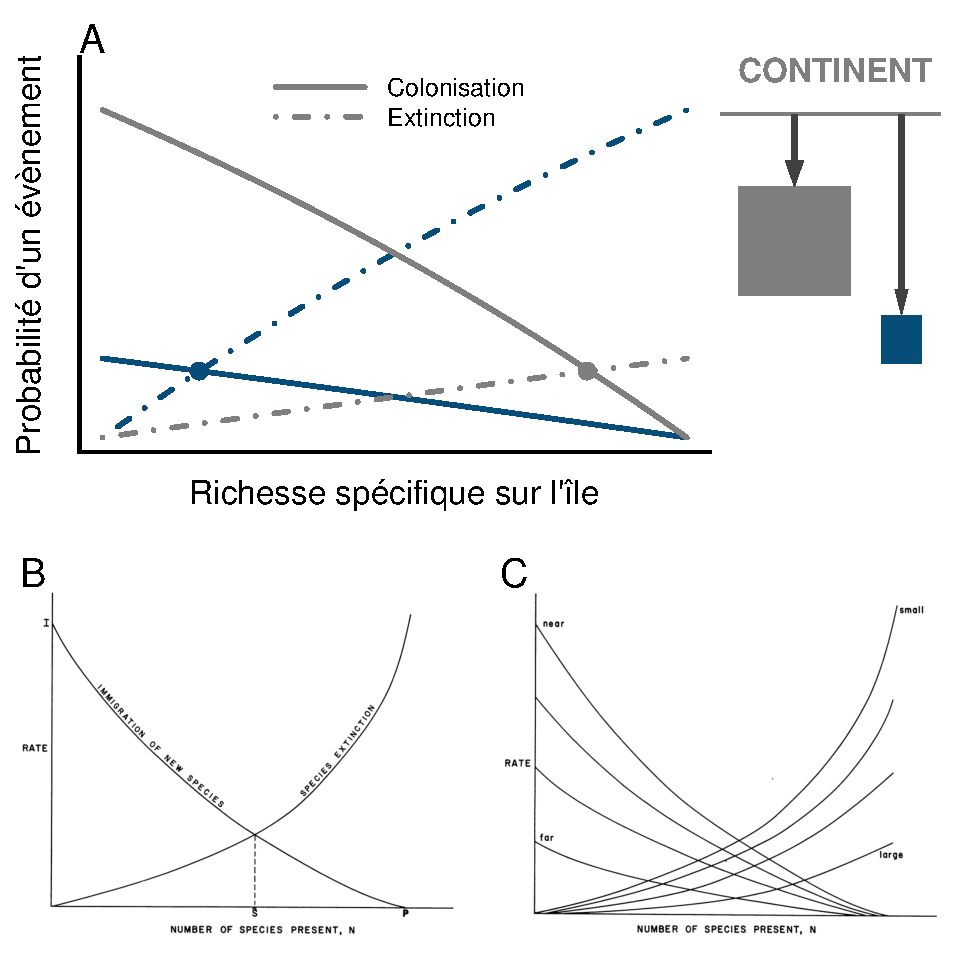
\includegraphics[width=0.80000\textwidth]{fig/fig1.pdf}
\caption{Une petite figure\label{fig:intr1}}
\end{figure}

Pour faire une référence à la figure \ref{fig:intr1}. Pour ce faire
j'utilise \href{https://github.com/tomduck/pandoc-fignos}{Pandoc-fignos}

\subsection*{Tables}\label{tables}
\addcontentsline{toc}{subsection}{Tables}

Pour les utilisateurs de R, une astuce: faîtes vos tables avec R et
utiliser la fonction \texttt{kable} du package
\href{http://yihui.name/knitr/}{knitr}!

\begin{longtable}[]{@{}llllrr@{}}
\caption{Une petite légende. \label{tbl:intr_1}}\tabularnewline
\toprule
& Plant & Type & Treatment & conc & uptake\tabularnewline
\midrule
\endfirsthead
\toprule
& Plant & Type & Treatment & conc & uptake\tabularnewline
\midrule
\endhead
8 & Qn2 & Quebec & nonchilled & 95 & 13.6\tabularnewline
16 & Qn3 & Quebec & nonchilled & 175 & 32.4\tabularnewline
24 & Qc1 & Quebec & chilled & 250 & 30.3\tabularnewline
32 & Qc2 & Quebec & chilled & 350 & 38.8\tabularnewline
40 & Qc3 & Quebec & chilled & 500 & 38.9\tabularnewline
48 & Mn1 & Mississippi & nonchilled & 675 & 32.4\tabularnewline
56 & Mn2 & Mississippi & nonchilled & 1000 & 31.5\tabularnewline
64 & Mc1 & Mississippi & chilled & 95 & 10.5\tabularnewline
72 & Mc2 & Mississippi & chilled & 175 & 11.4\tabularnewline
80 & Mc3 & Mississippi & chilled & 250 & 17.9\tabularnewline
\bottomrule
\end{longtable}

Pour faire des références aux tables j'utilise
\href{https://github.com/tomduck/pandoc-tablenos}{pandoc-tablenos} Et
hop je vaos référence à la figured \ref{tbl:intr_1}.

\subsection*{Références
bibliographiques}\label{ruxe9fuxe9rences-bibliographiques}
\addcontentsline{toc}{subsection}{Références bibliographiques}

Pour faire une référence en ligne \citet{Cazelles2016a}; une citation
entre parenthèse \citep{Cazelles2016a}; une citation avec du texte entre
parenthèse \citep[voir][]{Cazelles2016a}. Une succession de citation
\citep{Cazelles2016a, MacArthur1967, DeRuiter1995}.

Références aux autres chapitre. Il faut définir des labels et puis
simplement les appeller en utiisant les \textbackslash{}ref\{chap1\}. Au
chapitre \ref{chap1}, je fais un truc super.

\subsection*{Inclure du code}\label{inclure-du-code}
\addcontentsline{toc}{subsection}{Inclure du code}

Dans une ligne \texttt{x\ \textless{}-\ 3} et pour inclure du code sous
la forme d'un bloc~:

\begin{Shaded}
\begin{Highlighting}[]
\ControlFlowTok{for}\NormalTok{ (i }\ControlFlowTok{in} \DecValTok{1}\OperatorTok{:}\DecValTok{10}\NormalTok{)\{}
  \KeywordTok{print}\NormalTok{(i)}
\NormalTok{\}}
\end{Highlighting}
\end{Shaded}

\begin{Shaded}
\begin{Highlighting}[]
\KeywordTok{for} \ExtensionTok{i}\NormalTok{ in }\KeywordTok{`}\FunctionTok{seq}\NormalTok{ 1 6}\KeywordTok{`;} \KeywordTok{do} \ExtensionTok{qsub}\NormalTok{ start}\VariableTok{$i}\NormalTok{.sh }\KeywordTok{;} \KeywordTok{done}
\end{Highlighting}
\end{Shaded}


\cleardoublepage


\selectlanguage{english}

\chapter{TITRE CHAPITRE 1}
\label{chap1}

\section{Résumé en français du deuxième article}

\subsection{Contexte scientifique}

\subsection{Publication}
\subsection{Introduction}\label{introduction}

\subsection{Mat \& Meth}\label{mat-meth}

\begin{figure}[htbp]
\centering
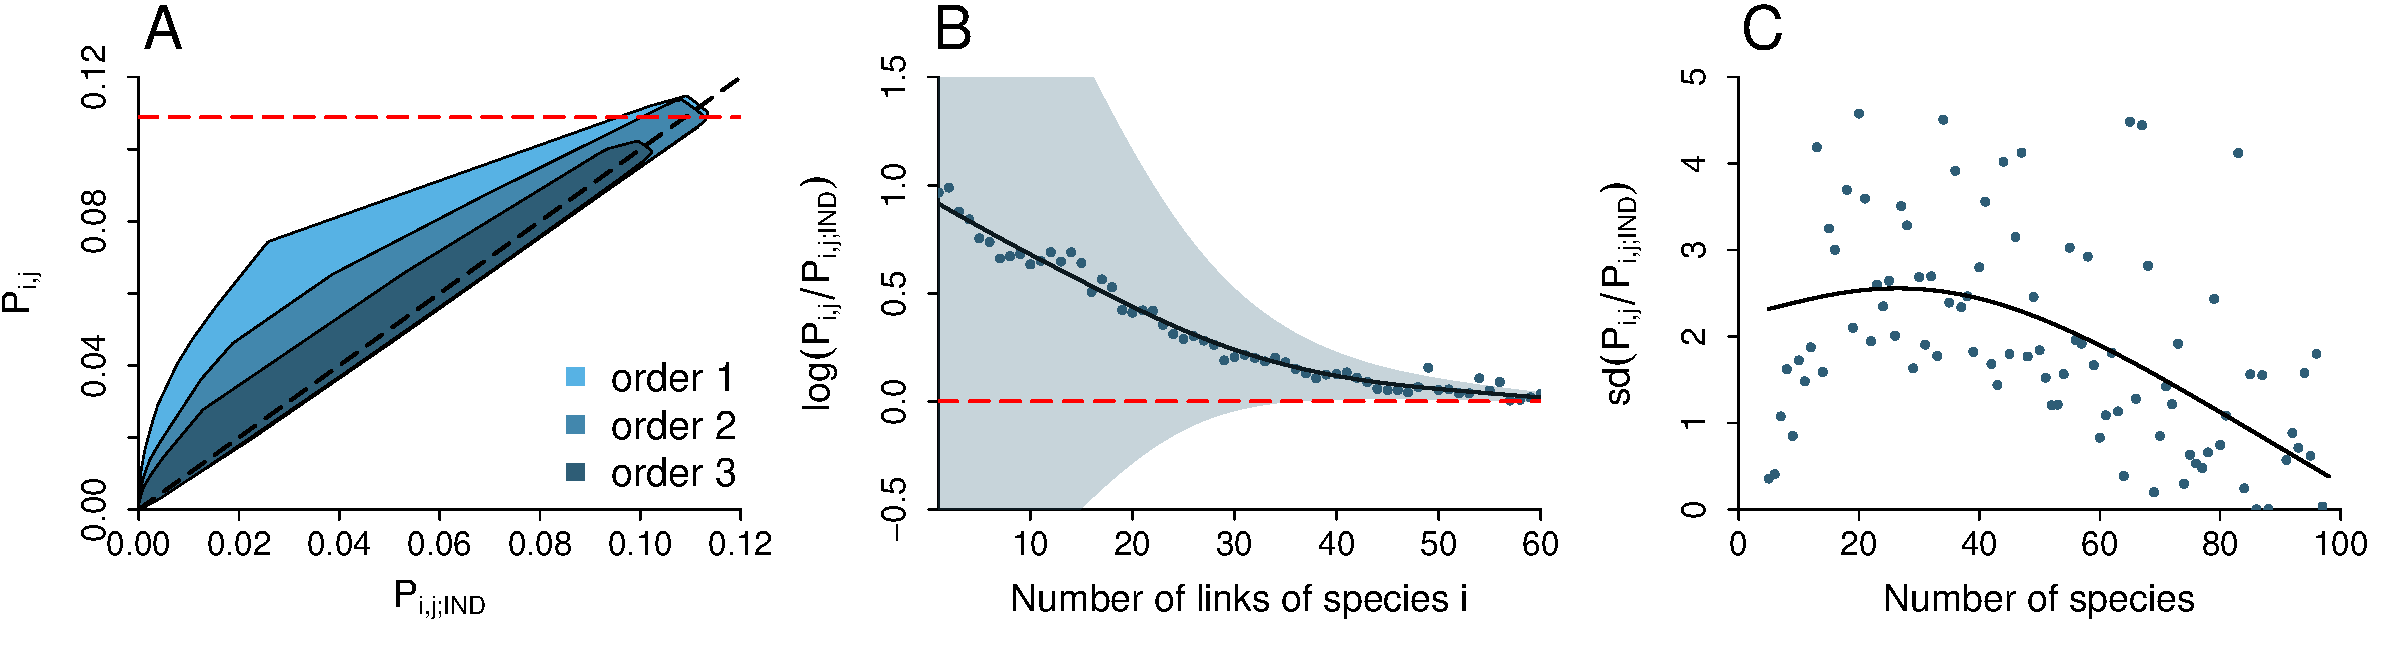
\includegraphics[width=\textwidth]{chapitre1/fig/fig1.eps}
\caption{Une belle figure\label{fig:chap1_1}}
\end{figure}

Vais faire une ref à la figure \ref{fig:chap1_1}

\chapter{TITRE CHAPITRE 2}
\label{chap2}

\section{Résumé en français du deuxième article}

\subsection{Contexte scientifique}

\subsection{Publication}


\emph{Les sections qui suivent sont celles de l'article publié.}


\section{Title}\label{title}


\section{Abstract}\label{abstract}


\section{Introduction}\label{introduction}

\chapter{TITRE CHAPITRE 3}
\label{chap3}

\section{Résumé en français du troisième article}

\subsection{Contexte scientifique}

\subsection{Publication}


\emph{Les sections qui suivent sont celles de l'article publié.}


\section{Title}\label{title}


\section{Abstract}\label{abstract}


\section{Introduction}\label{introduction}


\cleardoublepage


\conclusion
\selectlanguage{french}
\section*{Une belle conclusion
générale}\label{une-belle-conclusion-guxe9nuxe9rale}
\addcontentsline{toc}{section}{Une belle conclusion générale}

Une petite conclusion générale du même format que l'introduction

\subsection*{Prout}\label{prout}
\addcontentsline{toc}{subsection}{Prout}

\cleardoublepage




% ----------------------------------------------------------------------%
% 4 - Appendices de la thèse.                                           %
% ----------------------------------------------------------------------%


\selectlanguage{french}
\appendice{Comment la biodiversité s'installe en territoires isolés}
\label{annI}
\addtocounter{chapter}{1}
\setcounter{equation}{0}


\section{Présenter son annexe}

C'est l'annexe 1


\section{Mega cool}

\selectlanguage{english}
\appendice{Un modèle stochastique de la biogéographie insulaire pour les
réseaux écologiques dans un environnement abiotique variable}
\label{annII}
\addtocounter{chapter}{1}
\setcounter{equation}{0}
% \title{Supplemental material: \\ an integrative island biogeography model for ecological networks in a changing environment}

\section{Présenter son annexe 2}

\section{Mega cool}







% ----------------------------------------------------------------------%
% 5 - Bibliographie.                                                    %
% ----------------------------------------------------------------------%

\selectlanguage{english}

\begin{singlespace}
  \makeatletter
  \phantomsection\addcontentsline{toc}{chapter}{\MakeUppercase{\@references}}
  \makeatother
  \bibliographystyle{apalike}
  \bibliography{mybiblio} % Ici mettre le nom de la biblio, ici mylib.bib
\end{singlespace}

% \begin{singlespace}
%   \makeatletter
%   \phantomsection\addcontentsline{toc}{chapter}{\MakeUppercase{\@references}}
%   \makeatother
%   \selectlanguage{english}
%   % \bibliographystyle{elsevier-harvard.csl} % Ici éditer le style
%   \bibliography{/Users/KevCaz/Documents/library.bib} % Ici mettre le nom de la biblio, ici mylib.bib
% \end{singlespace}



% ----------------------------------------------------------------------%
% Fin du document.                                                     %
% ----------------------------------------------------------------------%

\end{document}
